% ============================================================
% M3 S2 导学件·波1 臂1 片件 —— 课时02（2.2.1 直线的倾斜角与斜率·上）
% 生成：M3 成卷轮 S2 波1臂1 量产代理｜2026-09-14｜编译 cwd＝本目录（中文路径禁 \input 绝对路径）
%   xelatex main-true.tex ×2 → 含详解印本；xelatex main-false.tex ×2 → 纯题版（单源双本）
% 输入链（全只读）：题面库 课时02-倾斜角与斜率.md（题面逐字装配）
%   ＋ 课时02-倾斜角与斜率-答案侧.md（值逐字回嵌）＋ 定稿/批A-课时02-倾斜角与斜率.md
%   （详解回嵌源 §一/§二/§三）；toolchain＝qp-m3.sty（md5 7c3930362be8a0a2bdf21bbf8ac16573，
%   本地挂载副本，禁改；破损即停）。
% 母版体例：承《课时01-坐标法/母版体例说明.md》——课前预习（知识点填空＋判断正误＋书写位，
%   零键零答案）→ 课中探究（4 考点×例＋变式＝20 键）→ 课堂检测 G5（3单选＋2填空）→ 尾块。
% 键账：件内 ansblock 键集 ≡ 题面库片键集 ≡ manifest 键序（25 键＝E16＋T4＋G5，零缺漏零多余）；
%   印面号 1—20＝考点探究（例/变式装配序）＋21—25＝课堂检测 G1—G5；键↔号映射见
%   值台账-课时02.json。多选 1 道（E6，全件 ≤2 合规）。
% 括线判据（承重墙禁放宽）：块内容估高＞8 行（wlen/23 栏宽口径，逐键读数入台账）→ 括线模。
% 图债登记：E1（国旗五星）已于 0914 S4 插桩销案（\ansfig 40mm 在题面「如图」处，figs/02-E1.png）。
% 门谱读数：见 过程件 工作区/_tmpM3S2波1臂1_0914/（编译 log、门谱输出、目验）。
% ============================================================
\documentclass[fontset=none]{ctexart}
\usepackage{qp-m3}
% —— 印面逐字符号路由补钉（探针实证 0914：书宋缺 U+2212，▱ 诸字库皆缺→NSC 子块；
%     禁改 sty 本体保 md5；无 ▱/− 用件的片可整块照抄，零副作用） ——
\xeCJKDeclareCharClass{Default}{"2212}%
\setCJKfamilyfont{nscblk}[Path=C:/提示词/工作区/字替对照-0909/variantF/fonts/,BoldFont=NSC-w600.ttf]{NSC-w500.ttf}%
\xeCJKDeclareSubCJKBlock{nscblk}{"25B1}%
\newcommand{\pxparallelogram}{{\CJKfamily{nscblk}▱}}%
% —— 断行微调（纯题档/详解档三零门：CJK 胶收缩 0.01→0.05em；伸展分量本件按数学密集
%     详解实测由 0.08em 放宽至 0.25em——胶点稀的公式行需更大伸展量才能撑满栏宽，
%     否则 Underfull \hbox；只动伸缩分量不动自然宽度，版面纹理零漂） ——
\xeCJKsetup{CJKglue={\hskip 0.10em plus 0.25em minus 0.05em}}%
% —— 页脚件名（qp-headfoot 复用入口） ——
\renewcommand{\qpzhangming}{第二章\quad 平面解析几何}%
\renewcommand{\qpjianming}{导学件}%

\begin{document}
%装配轮S6三本跨本连续页码（G7方案B）setcounter 注入位
\setcounter{page}{13}

\zhangtitle{第二章\quad 平面解析几何}
\jietitle{2.2.1 直线的倾斜角与斜率（第1课时）}
\mubiaoline
\mubiaomu{1}{理解倾斜角的概念及其“向上方向”的规定，掌握倾斜角的取值范围，会求给定直线的倾斜角；}
\mubiaomu{2}{理解斜率的定义，掌握两点间斜率公式，会由两点坐标求斜率并判断斜率的存在性；}
\mubiaomu{3}{理解倾斜角与斜率的对应关系，会由斜率的取值范围反求倾斜角的取值范围，体会数形结合的思想方法.}

\vspace{1.7mm}
\begin{multicols}{2}
\emergencystretch=1em

% ============================================================
% 课前预习（知识点填空＋判断正误＝件侧自教材 §2.2.1 组织，非题库题；零键零答案，
% \kongbai 空线两档等形不泄答）
% ============================================================
\huaxing{课}{前}{预}{习}{知识导学\quad 素养初识}

\zsd{一}{倾斜角}

\tiaomu{1}{在平面直角坐标系中，对于一条直线 \(l\)，\kongbai{}叫做直线 \(l\) 的倾斜角．规定：直线与 \(x\) 轴平行或重合时，倾斜角为\kongbai{}．\zhuzhu{倾斜角刻画直线的"倾斜程度"，是"向上方向"与 \(x\) 轴正方向所成的角，只看方向不看位置.}}

\tiaomu{2}{倾斜角 \(\alpha\) 的取值范围是\kongbai{}．\zhuzhu{开区间右端取不到：\(\alpha=180^{\circ}\) 与 \(\alpha=0^{\circ}\) 表示同一直线方向，故归入 \(0^{\circ}\).}}

\zsd{二}{斜率的定义与两点斜率公式}

\tiaomu{1}{直线倾斜角 \(\alpha\)（\(\alpha\neq 90^{\circ}\)）的\kongbai{}叫做这条直线的斜率，即 \(k=\)\kongbai{}；倾斜角为 \(90^{\circ}\) 的直线斜率\kongbai{}．\zhuzhu{斜率存在与否由倾斜角是否为 \(90^{\circ}\) 决定，这是概念辨析题的第一道关.}}

\tiaomu{2}{经过两点 \(P_1(x_1,y_1)\)、\(P_2(x_2,y_2)\)（\(x_1\neq x_2\)）的直线斜率为 \(k=\)\kongbai{}；若 \(x_1=x_2\)，则直线\kongbai{}，斜率不存在．\zhuzhu{公式与两点顺序无关（分子分母同时变号）；含参时用公式须先排除横坐标相等的情形.}}

\zsd{三}{倾斜角与斜率的关系}

\tiaomu{1}{\(\alpha\in[0^{\circ},90^{\circ})\) 时 \(k=\tan\alpha\geqslant 0\) 且随 \(\alpha\) 增大而\kongbai{}；\(\alpha\in(90^{\circ},180^{\circ})\) 时 \(k<0\) 且随 \(\alpha\) 增大而\kongbai{}．\zhuzhu{两段内各自递增，整体上"角大斜率大"不成立；由斜率范围回求倾斜角范围，须在 \([0,\pi/2)\) 与 \((\pi/2,\pi)\) 内分别取反正切再并集.}}

\zhenhead{判断正误(正确的打\gou{},错误的打\cha{})}

\zhentib{(1)}{任意一条直线都有倾斜角，也都有斜率．}

\zhentib{(2)}{直线的倾斜角越大，它的斜率就越大．}

\zhentib{(3)}{若两直线的斜率相等，则它们的倾斜角相等．}

\zhentib{(4)}{若直线的斜率为 \(\tan\alpha\)，则它的倾斜角就是 \(\alpha\)．}

\liubai[9mm]{此处书写}

% ============================================================
% 课中探究（考点探究〔例+变式〕＝练/拓槽 20 键；题后紧跟答案＝ansblock 内嵌，
% 值照答案侧逐字，详解承批A定稿回嵌＋印面清洗：〔〕→（）、provenance 括注剔除，
% 教学性括注（注意/易错/合理性）保留；纯文本数学式→\(...\) 换算入台账清洗注记）
% ============================================================
\huaxing{课}{中}{探}{究}{考点探究\quad 素养小结}

% ---------- 探究点一 倾斜角的概念与求角 ----------
\tjdnr{一}{倾斜角的概念与求角}{例\textbf{1}}{中档(知识点一)}{2020年12月4日，嫦娥五号探测器在月球表面第一次动态展示国旗．1949年公布的《国旗制法说明》中就五星的位置规定：大五角星有一个角尖正向上方，四颗小五角星均各有一个角尖正对大五角星的中心点．有人发现，第三颗小星的姿态与大星相近．为便于研究，如图，以大星的中心点为原点，建立直角坐标系，\(OO_1\)、\(OO_2\)、\(OO_3\)、\(OO_4\) 分别是大星中心点与四颗小星中心点的联结线，\(\alpha\approx 16^{\circ}\)，则第三颗小星的一条边 \(AB\) 所在直线的倾斜角约为\nobreak(\kongwei)}
\ansfig{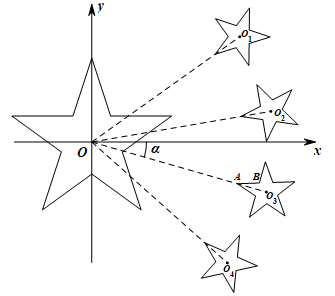
\includegraphics[width=40mm]{figs/02-E1.png}}

\bindopt {\fontsize{10.5pt}{\qpTJgLeadLiti}\selectfont \makebox[\dimexpr0.5\linewidth-1em\relax][l]{A．\(0^{\circ}\)}\makebox[\dimexpr0.5\linewidth-1em\relax][l]{B．\(1^{\circ}\)}\par}
\bindopt {\fontsize{10.5pt}{\qpTJgLeadLiti}\selectfont \makebox[\dimexpr0.5\linewidth-1em\relax][l]{C．\(2^{\circ}\)}\makebox[\dimexpr0.5\linewidth-1em\relax][l]{D．\(3^{\circ}\)}\par}

\begin{ansblock}[2章-练-课时02-E1]
% ans:2章-练-课时02-E1
\ansitem{1}{C}
\ansnote{详解}{\(O\)、\(O_3\) 都为五角星的中心点，故 \(OO_3\) 平分第三颗小星的一个角；又五角星的内角为 \(36^{\circ}\)，可知\(\angle BAO_3=18^{\circ}\)．过 \(O_3\) 作 \(x\) 轴的平行线 \(O_3E\)，则\(\angle OO_3E=\alpha\approx 16^{\circ}\)，所以直线 \(AB\) 的倾斜角约为 \(18^{\circ}-16^{\circ}=2^{\circ}\)，选C．}
\end{ansblock}

\liB{变式\textbf{2}}{简单(知识点一)}{}{直线\(2x\cdot\sin 210^{\circ}-y-2=0\)的倾斜角是\nobreak(\kongwei)}

\bindopt {\fontsize{10.5pt}{\qpTJgLeadLiti}\selectfont \makebox[\dimexpr0.5\linewidth-1em\relax][l]{A．\(45^{\circ}\)}\makebox[\dimexpr0.5\linewidth-1em\relax][l]{B．\(135^{\circ}\)}\par}
\bindopt {\fontsize{10.5pt}{\qpTJgLeadLiti}\selectfont \makebox[\dimexpr0.5\linewidth-1em\relax][l]{C．\(30^{\circ}\)}\makebox[\dimexpr0.5\linewidth-1em\relax][l]{D．\(150^{\circ}\)}\par}

\begin{ansblock}[2章-练-课时02-E9]
% ans:2章-练-课时02-E9
\ansitem{2}{B}
\ansnote{详解}{\(\sin 210^{\circ}=-1/2\)，直线方程即\(-x-y-2=0\)，即\(y=-x-2\)，斜率\(k=2\sin 210^{\circ}=-1\)，故倾斜角为 \(135^{\circ}\)，选B．}
\end{ansblock}

\liB{变式\textbf{3}}{简单(知识点一)}{}{已知直线\(l_1\)的倾斜角为\(30^{\circ}\)，直线\(l_2\)与\(l_1\)垂直，求直线\(l_2\)的倾斜角．}
\xiexwei{12mm}

\begin{ansblock}[2章-练-课时02-E15]
% ans:2章-练-课时02-E15
\ansitem{3}{120°}
\ansnote{详解}{\(l_2\) 与 \(l_1\) 垂直，则 \(l_2\) 的向上方向与 \(x\) 轴正向所成的角为\(30^{\circ}+90^{\circ}=120^{\circ}\)（在 \(l_2\) 向上方向取与 \(l_1\) 垂直且指向左上的一侧，另一直线方向与之共线）．由倾斜角的定义及\(0^{\circ}\leqslant\alpha<180^{\circ}\)，得 \(l_2\) 的倾斜角为\(120^{\circ}\)．（说明：两直线垂直时倾斜角关系的斜率判据在§2.2.3学习，本题只需用平面几何角的运算作答．）}
\end{ansblock}

\liB{变式\textbf{4}}{简单(知识点一)}{}{分别求下列直线的倾斜角：（1）\(y=\sqrt{3}x-2\)；（2）\(x+\sqrt{3}y+1=0\)；（3）\(x=-3\)；（4）\(y=1/2\)．}
\xiexwei{14mm}

\begin{ansblock}[2章-练-课时02-E16]
% ans:2章-练-课时02-E16
\ansitem{4}{(1) 60°；(2) 150°；(3) 90°；(4) 0°．}
\ansnote{详解}{（1）\(k=\sqrt{3}\)，\(\tan\alpha=\sqrt{3}\)，\(\alpha=60^{\circ}\)；（2）化为\(y=-(\sqrt{3}/3)x-\sqrt{3}/3\)，\(k=-\sqrt{3}/3\)，\(\tan\alpha=-\sqrt{3}/3\)，\(\alpha=150^{\circ}\)；（3）直线垂直于 \(x\) 轴，斜率不存在，倾斜角\(\alpha=90^{\circ}\)；（4）直线与 \(x\) 轴平行，倾斜角\(\alpha=0^{\circ}\)．}
\end{ansblock}

\xiaojie{①识别：凡"求倾斜角"，先定斜率（或斜率不存在）再用 \(\tan\alpha=k\) 在\([0^{\circ},180^{\circ})\) 内取角.②易错：\(k<0\) 时 \(\alpha\) 为钝角，\(\alpha=180^{\circ}-\arctan|k|\)，不可直接取负角.③通法：斜率不存在的直线（垂直 \(x\) 轴）倾斜角恒为 \(90^{\circ}\)．}

% ---------- 探究点二 斜率的定义与两点斜率公式 ----------
\tjdnr{二}{斜率的定义与两点斜率公式}{例\textbf{5}}{简单(知识点二)}{若\(A(-2,3)\)，\(B(3,2)\)，\(C(1/2,m)\)三点共线，则实数\(m\)的值为\nobreak(\kongwei)}

\bindopt {\fontsize{10.5pt}{\qpTJgLeadLiti}\selectfont \makebox[\dimexpr0.5\linewidth-1em\relax][l]{A．\(2\)}\makebox[\dimexpr0.5\linewidth-1em\relax][l]{B．\(-2\)}\par}
\bindopt {\fontsize{10.5pt}{\qpTJgLeadLiti}\selectfont \makebox[\dimexpr0.5\linewidth-1em\relax][l]{C．\(5/2\)}\makebox[\dimexpr0.5\linewidth-1em\relax][l]{D．\(-1/2\)}\par}

\begin{ansblock}[2章-练-课时02-E7]
% ans:2章-练-课时02-E7
\ansitem{5}{C}
\ansnote{详解}{三点共线\(\iff k_{AB}=k_{AC}\)．\(k_{AB}=(2-3)/(3+2)=-1/5\)；\(k_{AC}=(m-3)/(1/2+2)=(m-3)/(5/2)=2(m-3)/5\)．令\(2(m-3)/5=-1/5\)，得\(2(m-3)=-1\)，\(m=5/2\)，选C．}
\end{ansblock}

\liB{变式\textbf{6}}{简单(知识点二)}{}{已知经过\(A(a,-1)\)、\(B(2,a+1)\)的直线的斜率为\(3\)，求实数\(a\)的值．}
\xiexwei{10mm}

\begin{ansblock}[2章-练-课时02-E14]
% ans:2章-练-课时02-E14
\ansitem{6}{a＝1}
\ansnote{详解}{由斜率公式\(k=[(a+1)-(-1)]/(2-a)=(a+2)/(2-a)=3\)（须\(a\neq 2\)），去分母得\(a+2=3(2-a)=6-3a\)，\(4a=4\)，\(a=1\)，且\(a=1\neq 2\)满足条件．所以\(a=1\)．}
\end{ansblock}

\liB{变式\textbf{7}}{简单(知识点二)}{}{若\(A(3,1)\)，\(B(-2,k)\)，\(C(8,1)\)三点能构成三角形，则实数\(k\)的取值范围为\kongbai{}．}
\xiexwei{10mm}

\begin{ansblock}[2章-练-课时02-E10]
% ans:2章-练-课时02-E10
\ansitem{7}{(−∞,1)∪(1,+∞)}
\ansnote{详解}{三点能构成三角形\(\iff\)三点不共线．由\(k_{AB}\neq k_{AC}\)，即\((k-1)/(-2-3)\neq(1-1)/(8-3)\)，得\((k-1)/(-5)\neq 0\)，\(k-1\neq 0\)，\(k\neq 1\)．故\(k\)的取值范围为\((-\infty,1)\cup(1,+\infty)\)．}
\end{ansblock}

\liB{变式\textbf{8}}{简单(知识点二)}{\duoxuan\hspace{0.6em}}{若经过\(A(1-a,1+a)\)和\(B(3,a)\)的直线的倾斜角为钝角，则实数\(a\)的值可能为\nobreak(\kongwei)}

\bindopt {\fontsize{10.5pt}{\qpTJgLeadLiti}\selectfont \makebox[\dimexpr0.5\linewidth-1em\relax][l]{A．\(-2\)}\makebox[\dimexpr0.5\linewidth-1em\relax][l]{B．\(0\)}\par}
\bindopt {\fontsize{10.5pt}{\qpTJgLeadLiti}\selectfont \makebox[\dimexpr0.5\linewidth-1em\relax][l]{C．\(1\)}\makebox[\dimexpr0.5\linewidth-1em\relax][l]{D．\(2\)}\par}

\begin{ansblock}[2章-练-课时02-E6]
% ans:2章-练-课时02-E6
\ansitem{8}{BCD}
\ansnote{详解}{倾斜角为钝角\(\iff\)斜率存在且为负，即\(A\)、\(B\)横坐标不等且\(k_{AB}<0\)．\(k_{AB}=(1+a-a)/[(1-a)-3]=1/(-2-a)<0\)，得\(a+2>0\)，即\(a>-2\)．又\(a=-2\)时\(A(3,-1)\)、\(B(3,-2)\)横坐标相同、斜率不存在，倾斜角\(90^{\circ}\)，不在"钝角"取值内且\(a>-2\)已排除．故\(a>-2\)，选项中\(0\)、\(1\)、\(2\)满足，选BCD．}
\end{ansblock}

\liB{变式\textbf{9}}{简单(知识点二)}{}{已知两点\(A(1,-2)\)，\(B(2,1)\)，直线\(l\)过点\(P(0,-1)\)且与线段\(AB\)有交点，则直线\(l\)的斜率的取值范围为\nobreak(\kongwei)}

\bindopt {\fontsize{10.5pt}{\qpTJgLeadLiti}\selectfont \makebox[\dimexpr0.5\linewidth-1em\relax][l]{A．\([-1,1]\)}\makebox[\dimexpr0.5\linewidth-1em\relax][l]{B．\((-\infty,-1]\)}\par}
\bindopt {\fontsize{10.5pt}{\qpTJgLeadLiti}\selectfont \makebox[\dimexpr0.5\linewidth-1em\relax][l]{C．\((-1,1)\)}\makebox[\dimexpr0.5\linewidth-1em\relax][l]{D．\([1,+\infty)\)}\par}

\begin{ansblock}[2章-练-课时02-E2]
% ans:2章-练-课时02-E2
\ansitem{9}{A}
\ansnote{详解}{直线\(PA\)的斜率为\(k_{PA}=(-2+1)/(1-0)=-1\)，直线\(PB\)的斜率为\(k_{PB}=(1+1)/(2-0)=1\)．数形结合：当过\(P\)的直线\(l\)绕\(P\)从\(PA\)旋转到\(PB\)（保持与线段\(AB\)有公共点）时，其斜率介于\(k_{PA}\)与\(k_{PB}\)之间，故\(k\in[-1,1]\)，选A．}
\end{ansblock}

\liB{变式\textbf{10}}{简单(知识点二)}{}{直线\(m\)过点\(O(0,0)\)、\(A(1,\sqrt{2})\)，其倾斜角为\(\alpha\)，现将直线\(m\)绕原点\(O\)逆时针旋转得到直线\(m'\)：\(y=kx\)，若直线\(m'\)的倾斜角为\(2\alpha\)，则\(k\)的值为\nobreak(\kongwei)}

\bindopt {\fontsize{10.5pt}{\qpTJgLeadLiti}\selectfont \makebox[\dimexpr0.5\linewidth-1em\relax][l]{A．\(2\sqrt{2}\)}\makebox[\dimexpr0.5\linewidth-1em\relax][l]{B．\(-2\sqrt{2}\)}\par}
\bindopt {\fontsize{10.5pt}{\qpTJgLeadLiti}\selectfont \makebox[\dimexpr0.5\linewidth-1em\relax][l]{C．\(2\)}\makebox[\dimexpr0.5\linewidth-1em\relax][l]{D．\(-2\)}\par}

\begin{ansblock}[2章-练-课时02-E8]
% ans:2章-练-课时02-E8
\ansitem{10}{B}
\ansnote{详解}{\(\tan\alpha=k_{OA}=\sqrt{2}\)．\(m'\)的倾斜角为\(2\alpha\)，故\(k=\tan 2\alpha=2\tan\alpha/(1-\tan^{2}\alpha)=2\sqrt{2}/(1-2)=-2\sqrt{2}\)，选B．（合理性：\(\tan\alpha=\sqrt{2}>1\)，\(\alpha\in(\pi/4,\pi/2)\)，\(2\alpha\in(\pi/2,\pi)\)确为钝角，\(\tan 2\alpha<0\)．）}
\end{ansblock}

\xiaojie{①识别：给定两点坐标求斜率直接用\(k=(y_2-y_1)/(x_2-x_1)\)，含参时先列方程再检验分母不为零.②易错：三点共线要排除"横坐标相同"的竖直情形；由斜率符号定倾斜角钝锐.③通法：线段（或折线）上的动点与定点连线，斜率范围端点取在"过端点"处，先算两端再判连续．}

% ---------- 探究点三 倾斜角与斜率的互求 ----------
\tjdnr{三}{倾斜角与斜率的互求}{例\textbf{11}}{中档(知识点三)}{直线\(l\)的倾斜角为\(\alpha\)，且\(\sin\alpha=3/5\)，则直线\(l\)的斜率是\nobreak(\kongwei)}

\bindopt {\fontsize{10.5pt}{\qpTJgLeadLiti}\selectfont \makebox[\dimexpr0.5\linewidth-1em\relax][l]{A．\(-4/3\)}\makebox[\dimexpr0.5\linewidth-1em\relax][l]{B．\(3/4\)}\par}
\bindopt {\fontsize{10.5pt}{\qpTJgLeadLiti}\selectfont \makebox[\dimexpr0.5\linewidth-1em\relax][l]{C．\(3/4\)或\(-3/4\)}\makebox[\dimexpr0.5\linewidth-1em\relax][l]{D．\(4/3\)或\(-4/3\)}\par}

\begin{ansblock}[2章-练-课时02-E3]
% ans:2章-练-课时02-E3
\ansitem{11}{C}
\ansnote{详解}{\(\alpha\in[0^{\circ},180^{\circ})\)且\(\sin\alpha=3/5>0\)，故\(\alpha\)为锐角或钝角．当\(\alpha\)为锐角时\(\cos\alpha=4/5\)，\(k=\tan\alpha=3/4\)；当\(\alpha\)为钝角时\(\cos\alpha=-4/5\)，\(k=\tan\alpha=-3/4\)．故直线\(l\)的斜率是\(3/4\)或\(-3/4\)，选C．}
\end{ansblock}

\liB{变式\textbf{12}}{简单(知识点三)}{}{已知直线斜率为\(k\)，且\(-1\leqslant k\leqslant\sqrt{3}\)，那么倾斜角\(\alpha\)的取值范围是\nobreak(\kongwei)}

\bindopt {\fontsize{10.5pt}{\qpTJgLeadLiti}\selectfont \makebox[\dimexpr0.5\linewidth-1em\relax][l]{A．\([0,\pi/3]\cup[\pi/2,3\pi/4)\)}\makebox[\dimexpr0.5\linewidth-1em\relax][l]{B．\([0,\pi/3]\cup[3\pi/4,\pi)\)}\par}
\bindopt {\fontsize{10.5pt}{\qpTJgLeadLiti}\selectfont \makebox[\dimexpr0.5\linewidth-1em\relax][l]{C．\([0,\pi/6]\cup[\pi/2,3\pi/4)\)}\makebox[\dimexpr0.5\linewidth-1em\relax][l]{D．\([0,\pi/6]\cup[3\pi/4,\pi)\)}\par}

\begin{ansblock}[2章-练-课时02-E4]
% ans:2章-练-课时02-E4
\ansitem{12}{B}
\ansnote{详解}{\(\alpha\in[0,\pi)\)，\(-1\leqslant k\leqslant\sqrt{3}\)即\(-1\leqslant\tan\alpha\leqslant\sqrt{3}\)．当\(0\leqslant\tan\alpha\leqslant\sqrt{3}\)时\(\alpha\in[0,\pi/3]\)；当\(-1\leqslant\tan\alpha<0\)时\(\alpha\in[3\pi/4,\pi)\)．所以\(\alpha\in[0,\pi/3]\cup[3\pi/4,\pi)\)，选B．}
\end{ansblock}

\liB{变式\textbf{13}}{简单(知识点三)}{}{直线\(l\)经过点\(A(2,1)\)，\(B(3,t^{2})\)（\(-\sqrt{2}\leqslant t\leqslant\sqrt{2}\)），则直线\(l\)倾斜角的取值范围是\nobreak(\kongwei)}

\bindopt {\fontsize{10.5pt}{\qpTJgLeadLiti}\selectfont \makebox[\dimexpr0.5\linewidth-1em\relax][l]{A．\([0,\pi/4]\cup[3\pi/4,\pi)\)}\makebox[\dimexpr0.5\linewidth-1em\relax][l]{B．\([0,\pi/3]\cup[2\pi/3,\pi)\)}\par}
\bindopt {\fontsize{10.5pt}{\qpTJgLeadLiti}\selectfont \makebox[\dimexpr\linewidth-1em\relax][l]{C．\([\pi/4,\pi/2)\cup(\pi/2,3\pi/4]\)}\par}
\bindopt {\fontsize{10.5pt}{\qpTJgLeadLiti}\selectfont \makebox[\dimexpr\linewidth-1em\relax][l]{D．\([0,\pi/4]\)}\par}

\begin{ansblock}[2章-练-课时02-E5]
% ans:2章-练-课时02-E5
\ansitem{13}{A}
\ansnote{详解}{\(k_l=(t^{2}-1)/(3-2)=t^{2}-1\)．由\(-\sqrt{2}\leqslant t\leqslant\sqrt{2}\)得\(t^{2}\in[0,2]\)，故\(k\in[-1,1]\)，即\(\tan\theta\in[-1,1]\)（\(\theta\)为倾斜角），得\(\theta\in[0,\pi/4]\cup[3\pi/4,\pi)\)，选A．（注：本选项组为本卷补写——源题为无选项填空，为入选择槽按原题数据配四选项，答案为\(A\)不变．）}
\end{ansblock}

\liB{变式\textbf{14}}{简单(知识点三)}{}{若直线\(l\)的倾斜角的变化范围为\([\pi/6,\pi/3)\)，则直线斜率的取值范围是\kongbai{}．}
\xiexwei{10mm}

\begin{ansblock}[2章-练-课时02-E11]
% ans:2章-练-课时02-E11
\ansitem{14}{[√3/3, √3)}
\ansnote{详解}{正切函数\(k=\tan\alpha\)在\([\pi/6,\pi/3)\)上单调递增，故\(\alpha\in[\pi/6,\pi/3)\)时\(\tan\alpha\in[\tan(\pi/6),\tan(\pi/3))=[\sqrt{3}/3,\sqrt{3})\)，即斜率\(k\in[\sqrt{3}/3,\sqrt{3})\)．}
\end{ansblock}

\liB{变式\textbf{15}}{简单(知识点三)}{}{当直线\(l\)的倾斜角\(\theta\in[\pi/4,\pi/2)\cup(\pi/2,2\pi/3]\)时，直线\(l\)的斜率的取值范围为\kongbai{}．}
\xiexwei{10mm}

\begin{ansblock}[2章-练-课时02-E12]
% ans:2章-练-课时02-E12
\ansitem{15}{[1,+∞)∪(−∞,−√3]}
\ansnote{详解}{\(\theta\in[\pi/4,\pi/2)\)时，\(k=\tan\theta\in[\tan(\pi/4),+\infty)\)\allowbreak\(=[1,+\infty)\)\par\noindent \(\theta\in(\pi/2,2\pi/3]\)时，\(k=\tan\theta\in(-\infty,\tan(2\pi/3)]=(-\infty,-\sqrt{3}]\)\par\noindent 故\(k\)的取值范围为\([1,+\infty)\cup(-\infty,-\sqrt{3}]\)．}
\end{ansblock}

\liB{变式\textbf{16}}{简单(知识点三)}{}{已知直线\(l_1\)的斜率为\(-1\)，直线\(l_2\)的倾斜角比直线\(l_1\)的倾斜角小\(30^{\circ}\)，求直线\(l_2\)的斜率．}
\xiexwei{12mm}

\begin{ansblock}[2章-练-课时02-E13]
% ans:2章-练-课时02-E13
\ansitem{16}{−2−√3}
\ansnote{详解}{\(l_1\)的斜率为\(-1\)，其倾斜角为\(135^{\circ}\)，故\(l_2\)的倾斜角为\(135^{\circ}-30^{\circ}=105^{\circ}\)．\(k_2=\tan 105^{\circ}=\tan(60^{\circ}+45^{\circ})=(\tan 60^{\circ}+\tan 45^{\circ})/(1-\tan 60^{\circ}\cdot\tan 45^{\circ})=(\sqrt{3}+1)/(1-\sqrt{3})=(\sqrt{3}+1)^{2}/[(1-\sqrt{3})(1+\sqrt{3})]=(4+2\sqrt{3})/(-2)=-2-\sqrt{3}\)．所以直线\(l_2\)的斜率为\(-2-\sqrt{3}\)．}
\end{ansblock}

\xiaojie{①识别：角、率互求的"范围题"，先在\([0,\pi/2)\)与\((\pi/2,\pi)\)两段内各自取单调区间再并集.②易错：\(\tan\alpha=k\)由\(k\)反求\(\alpha\)时，\(k<0\)对应钝角，切勿写\(\alpha=\arctan k\)（负角）.③通法：含参斜率先求\(k\)的取值范围（换元、二次函数最值），再落到倾斜角的分段区间．}

% ---------- 探究点四 拓展·收难 ----------
\tjdnr{四}{拓展·收难}{例\textbf{17}}{中档(知识点三)}{（1）如果直线的倾斜角\(\theta\in[0,\pi/2)\)，则当\(\theta\)增大时，直线的斜率将怎样变化？如果\(\theta\in(\pi/2,\pi)\)呢？（2）能否说"直线的倾斜角增大时斜率也增大"？为什么？}
\xiexwei{14mm}

{\ansblockgrayfalse
\begin{ansblock}[2章-拓-课时02-T1]
% ans:2章-拓-课时02-T1
\ansitem{17}{(1) θ∈[0,π/2)时斜率由0递增并趋向＋∞；θ∈(π/2,π)时斜率由−∞递增趋向0；(2) 不能，理由见详解．}
\ansnote{详解}{（1）\(k=\tan\theta\)在\([0,\pi/2)\)上单调递增，\(k\)从\(0\)增大到正无穷大；在\((\pi/2,\pi)\)上也单调递增，\(k\)从负无穷大增大到\(0\)．（2）不能．例如取\(\theta_1=45^{\circ}\)，\(\theta_2=120^{\circ}\)，\(\theta_1<\theta_2\)，但\(k_1=1>k_2=-\sqrt{3}\)，即倾斜角大者斜率反而小；斜率关于倾斜角只在每一段\([0,\pi/2)\)与\((\pi/2,\pi)\)内分别递增，整体上不具有单调性．}
\end{ansblock}}

\liB{变式\textbf{18}}{中档(知识点二)}{}{已知坐标平面内三点\(A(-1,1)\)，\(B(1,1)\)，\(C(2,\sqrt{3}+1)\)．（1）求直线\(AB\)，\(BC\)，\(AC\)的斜率和倾斜角；（2）若\(D\)为\(\triangle ABC\)的\(AB\)边上一动点，求直线\(CD\)的倾斜角的取值范围．}
\xiexwei{16mm}

{\ansblockgrayfalse
\begin{ansblock}[2章-拓-课时02-T2]
% ans:2章-拓-课时02-T2
\ansitem{18}{(1) \(k_{AB}=0\)（倾斜角\(0\)）；\(k_{BC}=\sqrt{3}\)（倾斜角\(\pi/3\)）；\(k_{AC}=\sqrt{3}/3\)（倾斜角\(\pi/6\)）；(2) \([\pi/6,\ \pi/3]\)．}
\ansnote{详解}{（1）\(k_{AB}=(1-1)/(1+1)=0\)，\(k_{BC}=(\sqrt{3}+1-1)/(2-1)=\sqrt{3}\)，\(k_{AC}=(\sqrt{3}+1-1)/(2+1)=\sqrt{3}/3\)．因斜率等于倾斜角的正切值且倾斜角\(\alpha\in[0,\pi)\)，故\(AB\)、\(BC\)、\(AC\)的倾斜角依次为\(0\)、\(\pi/3\)、\(\pi/6\)．（2）当直线\(CD\)绕点\(C\)由\(CA\)逆时针旋转到\(CB\)时，\(CD\)与线段\(AB\)恒有交点（即\(D\)在\(AB\)上），此时\(k_{CD}\)由\(k_{AC}\)增大到\(k_{BC}\)，\(k_{CD}\in[\sqrt{3}/3,\sqrt{3}]\)，对应倾斜角\(\alpha\in[\pi/6,\pi/3]\)．}
\end{ansblock}}

\liB{变式\textbf{19}}{中档(知识点一)}{}{已知\(a\)，\(b\)，\(c\)是两两不相等的实数，分别求经过下列两点的直线的倾斜角：（1）\(A(a,c)\)，\(B(b,c)\)；（2）\(C(a,b)\)，\(D(a,c)\)；（3）\(P(b,b+c)\)，\(Q(a,c+a)\)．}
\xiexwei{14mm}

\begin{ansblock}[2章-拓-课时02-T3]
% ans:2章-拓-课时02-T3
\ansitem{19}{(1) 0°；(2) 90°；(3) 45°．}
\ansnote{详解}{（1）纵坐标同为\(c\)，直线与\(x\)轴平行，倾斜角为\(0^{\circ}\)（\(k=0\)）；（2）横坐标同为\(a\)，直线垂直于\(x\)轴，斜率不存在，倾斜角为\(90^{\circ}\)；（3）\(k=[(c+a)-(b+c)]/(a-b)=(a-b)/(a-b)=1\)（\(a\neq b\)），\(\tan\alpha=1\)，\(\alpha\in[0^{\circ},180^{\circ})\)，故倾斜角为\(45^{\circ}\)．}
\end{ansblock}

\liB{变式\textbf{20}}{难(知识点二)}{}{点\(M(x,y)\)在函数\(y=-2x+8\)的图象上，当\(x\in[2,5]\)时，求\((y+1)/(x+1)\)的取值范围．}
\xiexwei{10mm}

{\ansblockgrayfalse
\begin{ansblock}[2章-拓-课时02-T4]
% ans:2章-拓-课时02-T4
\ansitem{20}{[−1/6, 5/3]}
\ansnote{详解}{\((y+1)/(x+1)=[y-(-1)]/[x-(-1)]\)的几何意义是过\(M(x,y)\)与定点\(N(-1,-1)\)两点的直线的斜率，其中点\(M\)在线段\(y=-2x+8\)（\(x\in[2,5]\)）上运动．线段两端点为\((2,4)\)与\((5,-2)\)．记\(k(x)=(y+1)/(x+1)=(-2x+9)/(x+1)=-2+11/(x+1)\)，在\(x\in[2,5]\)上随\(x\)增大而单调递减，故最大值在\(x=2\)处取得：\(k=(4+1)/(2+1)=5/3\)；最小值在\(x=5\)处取得：\(k=(-2+1)/(5+1)=-1/6\)．所以\((y+1)/(x+1)\)的取值范围为\([-1/6,5/3]\)．}
\end{ansblock}}

\xiaojie{①识别：\((y-b)/(x-a)\)型最值＝"动点与定点连线斜率"，端点法或单调性二选一.②易错：绕定点旋转的斜率范围须先判是否跨过竖直位置，跨\(\pi/2\)时必分段.③通法：说理题（如"角大率大"）一律取反例，反例取在两段交界处最省力．}

% ============================================================
% 课堂检测（G5＝导学槽 5 键，印面号 21—25；3单选＋2填空，值照答案侧逐字）
% ============================================================
\begin{ketang}{本组共5题（第21—25题），21—23为单选，24—25为填空．}

\jiancestem{{\fontsize{11.4pt}{14pt}\selectfont\heihao {\numboldjian 21}．}\hspace{4.1mm}\tieside{简单}\hspace{2.2mm}若直线\(l\)的向上方向与\(y\)轴正方向成\(30^{\circ}\)角，则直线\(l\)的倾斜角为\nobreak(\kongwei)}

\bindopt {\fontsize{10.5pt}{\qpTJgLeadPingjia}\selectfont \makebox[\dimexpr0.5\linewidth-1em\relax][l]{A．\(30^{\circ}\)}\makebox[\dimexpr0.5\linewidth-1em\relax][l]{B．\(60^{\circ}\)}\par}
\bindopt {\fontsize{10.5pt}{\qpTJgLeadPingjia}\selectfont \makebox[\dimexpr0.5\linewidth-1em\relax][l]{C．\(30^{\circ}\)或\(150^{\circ}\)}\makebox[\dimexpr0.5\linewidth-1em\relax][l]{D．\(60^{\circ}\)或\(120^{\circ}\)}\par}

\begin{ansblock}[2章-导-课时02-G1]
% ans:2章-导-课时02-G1
\ansitem{21}{D}
\ansnote{详解}{直线\(l\)的向上方向与\(y\)轴正方向成\(30^{\circ}\)角，\(l\)有两种位置（偏左或偏右）：与\(x\)轴正方向所成的角可能为\(90^{\circ}-30^{\circ}=60^{\circ}\)或\(90^{\circ}+30^{\circ}=120^{\circ}\)，故\(l\)的倾斜角为\(60^{\circ}\)或\(120^{\circ}\)，选D．}
\end{ansblock}

\jiancestem{{\fontsize{11.4pt}{14pt}\selectfont\heihao {\numboldjian 22}．}\hspace{4.1mm}\tieside{简单}\hspace{2.2mm}下列说法中，正确的是\nobreak(\kongwei)}

\lxopt{A．直线的倾斜角为\(\alpha\)，则此直线的斜率为\(\tan\alpha\)}
\lxopt{B．直线的斜率为\(\tan\alpha\)，则此直线的倾斜角为\(\alpha\)}
\lxopt{C．若直线的倾斜角为\(\alpha\)，则\(\sin\alpha>0\)}
\lxopt{D．任意直线都有倾斜角\(\alpha\)，且\(\alpha\neq 90^{\circ}\)时，斜率为\(\tan\alpha\)}

\begin{ansblock}[2章-导-课时02-G2]
% ans:2章-导-课时02-G2
\ansitem{22}{D}
\ansnote{详解}{A：当\(\alpha=90^{\circ}\)时，直线的斜率不存在，故A不正确；B：虽然直线的斜率为\(\tan\alpha\)，但只有当\(0^{\circ}\leqslant\alpha<180^{\circ}\)时，\(\alpha\)才是此直线的倾斜角，故B不正确；C：当直线与\(x\)轴平行或重合时，\(\alpha=0^{\circ}\)，\(\sin\alpha=0\)，故C不正确；由倾斜角的定义（任意直线都有倾斜角，范围\(0^{\circ}\leqslant\alpha<180^{\circ}\)）与斜率的定义（\(\alpha\neq 90^{\circ}\)时\(k=\tan\alpha\)）知D正确，选D．}
\end{ansblock}

\jiancestem{{\fontsize{11.4pt}{14pt}\selectfont\heihao {\numboldjian 23}．}\hspace{4.1mm}\tieside{简单}\hspace{2.2mm}若两直线\(l_1\)，\(l_2\)的倾斜角和斜率分别为\(\alpha_1\)，\(\alpha_2\)和\(k_1\)，\(k_2\)，则下列四个命题中正确的是\nobreak(\kongwei)}

\lxopt{A．若\(\alpha_1<\alpha_2\)，则\(k_1<k_2\)}
\lxopt{B．若\(\alpha_1=\alpha_2\)，则\(k_1=k_2\)}
\lxopt{C．若\(k_1<k_2\)，则\(\alpha_1<\alpha_2\)}
\lxopt{D．若\(k_1=k_2\)，则\(\alpha_1=\alpha_2\)}

\begin{ansblock}[2章-导-课时02-G3]
% ans:2章-导-课时02-G3
\ansitem{23}{D}
\ansnote{详解}{A：取\(\alpha_1=45^{\circ}\)，\(\alpha_2=135^{\circ}\)，则\(k_1=1\)，\(k_2=-1\)，\(k_1>k_2\)，故A错误；B：取\(\alpha_1=\alpha_2=90^{\circ}\)，则\(k_1\)、\(k_2\)都不存在，故B错误；C：取\(k_1=-1\)，\(k_2=1\)，则\(\alpha_1=135^{\circ}\)，\(\alpha_2=45^{\circ}\)，\(\alpha_1>\alpha_2\)，故C错误；D：斜率相等即\(\tan\alpha_1=\tan\alpha_2\)，而\(\alpha_1\)、\(\alpha_2\in[0^{\circ},180^{\circ})\)且均不为\(90^{\circ}\)，正切值相等则角相等，D正确，选D．}
\end{ansblock}

\jiancestem{{\fontsize{11.4pt}{14pt}\selectfont\heihao {\numboldjian 24}．}\hspace{4.1mm}\tieside{简单}\hspace{2.2mm}分别写出下列直线的倾斜角：（1）垂直于\(x\)轴的直线；（2）垂直于\(y\)轴的直线；（3）第一、三象限的角平分线；（4）第二、四象限的角平分线．}
\xiexwei{8mm}

\begin{ansblock}[2章-导-课时02-G4]
% ans:2章-导-课时02-G4
\ansitem{24}{(1) 90°；(2) 0°；(3) 45°；(4) 135°．}
\ansnote{详解}{（1）与\(x\)轴垂直，倾斜角为\(90^{\circ}\)；（2）与\(x\)轴平行或重合，规定倾斜角为\(0^{\circ}\)；（3）角平分线\(y=x\)与\(x\)轴正方向成\(45^{\circ}\)角，倾斜角为\(45^{\circ}\)；（4）角平分线\(y=-x\)向上的方向与\(x\)轴正方向成\(135^{\circ}\)角，倾斜角为\(135^{\circ}\)．}
\end{ansblock}

\jiancestem{{\fontsize{11.4pt}{14pt}\selectfont\heihao {\numboldjian 25}．}\hspace{4.1mm}\tieside{简单}\hspace{2.2mm}已知直线\(l\)的倾斜角为\(2\alpha-20^{\circ}\)，则\(\alpha\)的取值范围是\kongbai{}．}
\xiexwei{8mm}

\begin{ansblock}[2章-导-课时02-G5]
% ans:2章-导-课时02-G5
\ansitem{25}{10°≤α＜100°}
\ansnote{详解}{由倾斜角的取值范围\(0^{\circ}\leqslant 2\alpha-20^{\circ}<180^{\circ}\)，各边加\(20^{\circ}\)再除以\(2\)，得\(10^{\circ}\leqslant\alpha<100^{\circ}\)．}
\end{ansblock}

\end{ketang}

% ---- 尾块（\tailfill 置 \end{multicols} 前；无参＝内容尾随框，件侧不擅自定高） ----
\tailfill

\end{multicols}
\end{document}
